\documentclass{article}
\usepackage[utf8]{inputenc}

%meer ams meer beter
\usepackage{amsmath}
\usepackage{amssymb}
\usepackage{amsthm} %nodig voor blokje

\usepackage{marginnote}
\usepackage[margin=1in,footskip=0.25in]{geometry} %heb wat meer ruimte

%Plaatjes
\usepackage{graphicx}
\usepackage{float}
\usepackage{caption}
\usepackage{subcaption}
\usepackage{epstopdf}

\begin{document}
\begin{figure}[h]
    \centering
<<<<<<< HEAD
    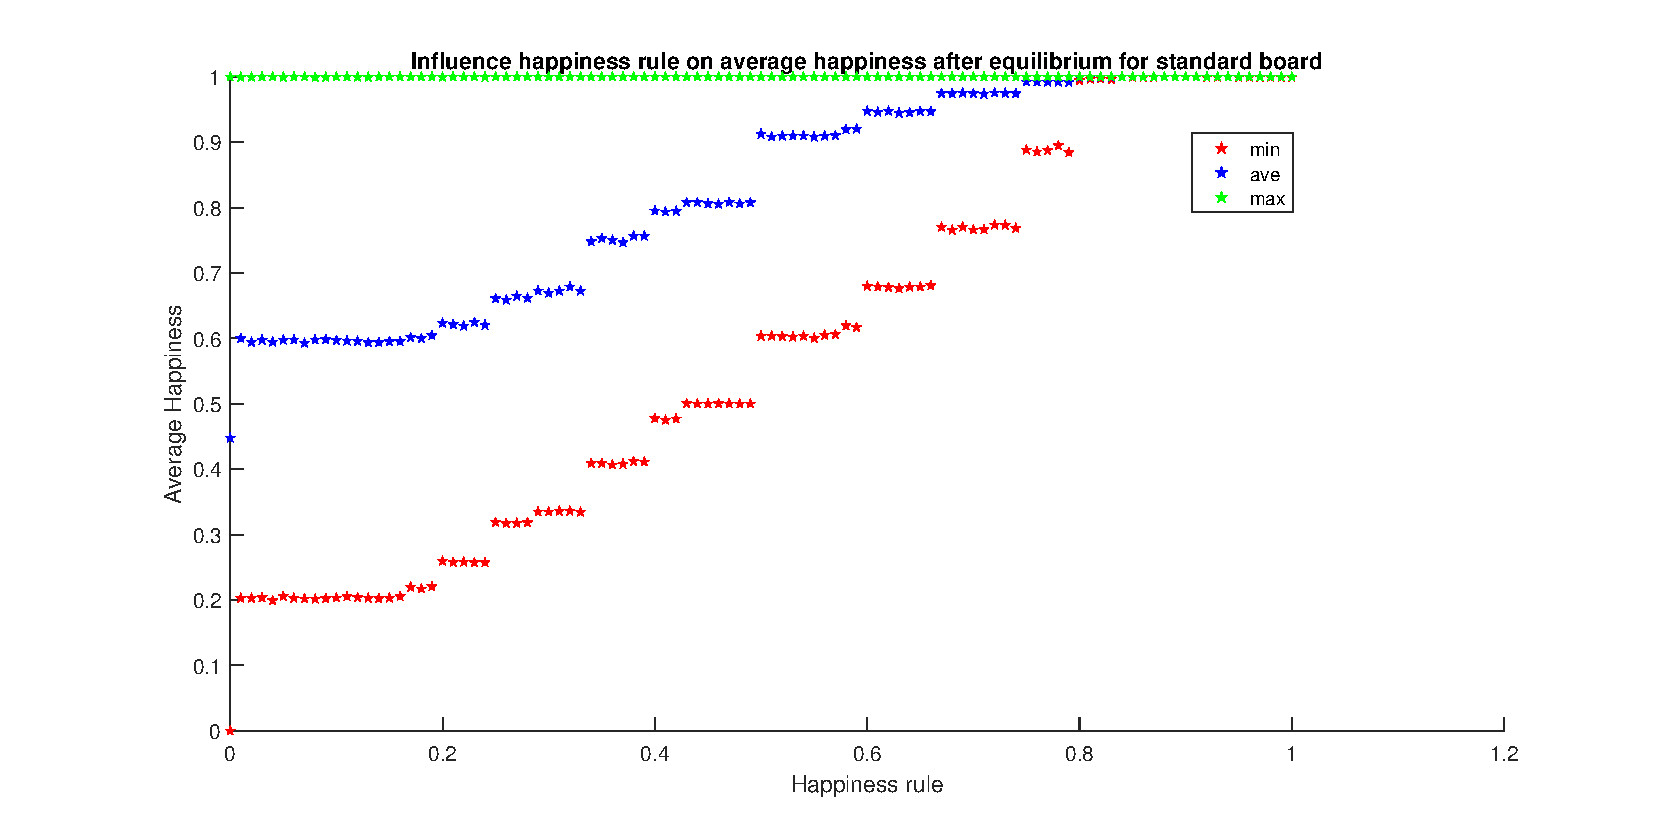
\includegraphics{happinessregel-gemhappinesseind-2.eps}
=======
    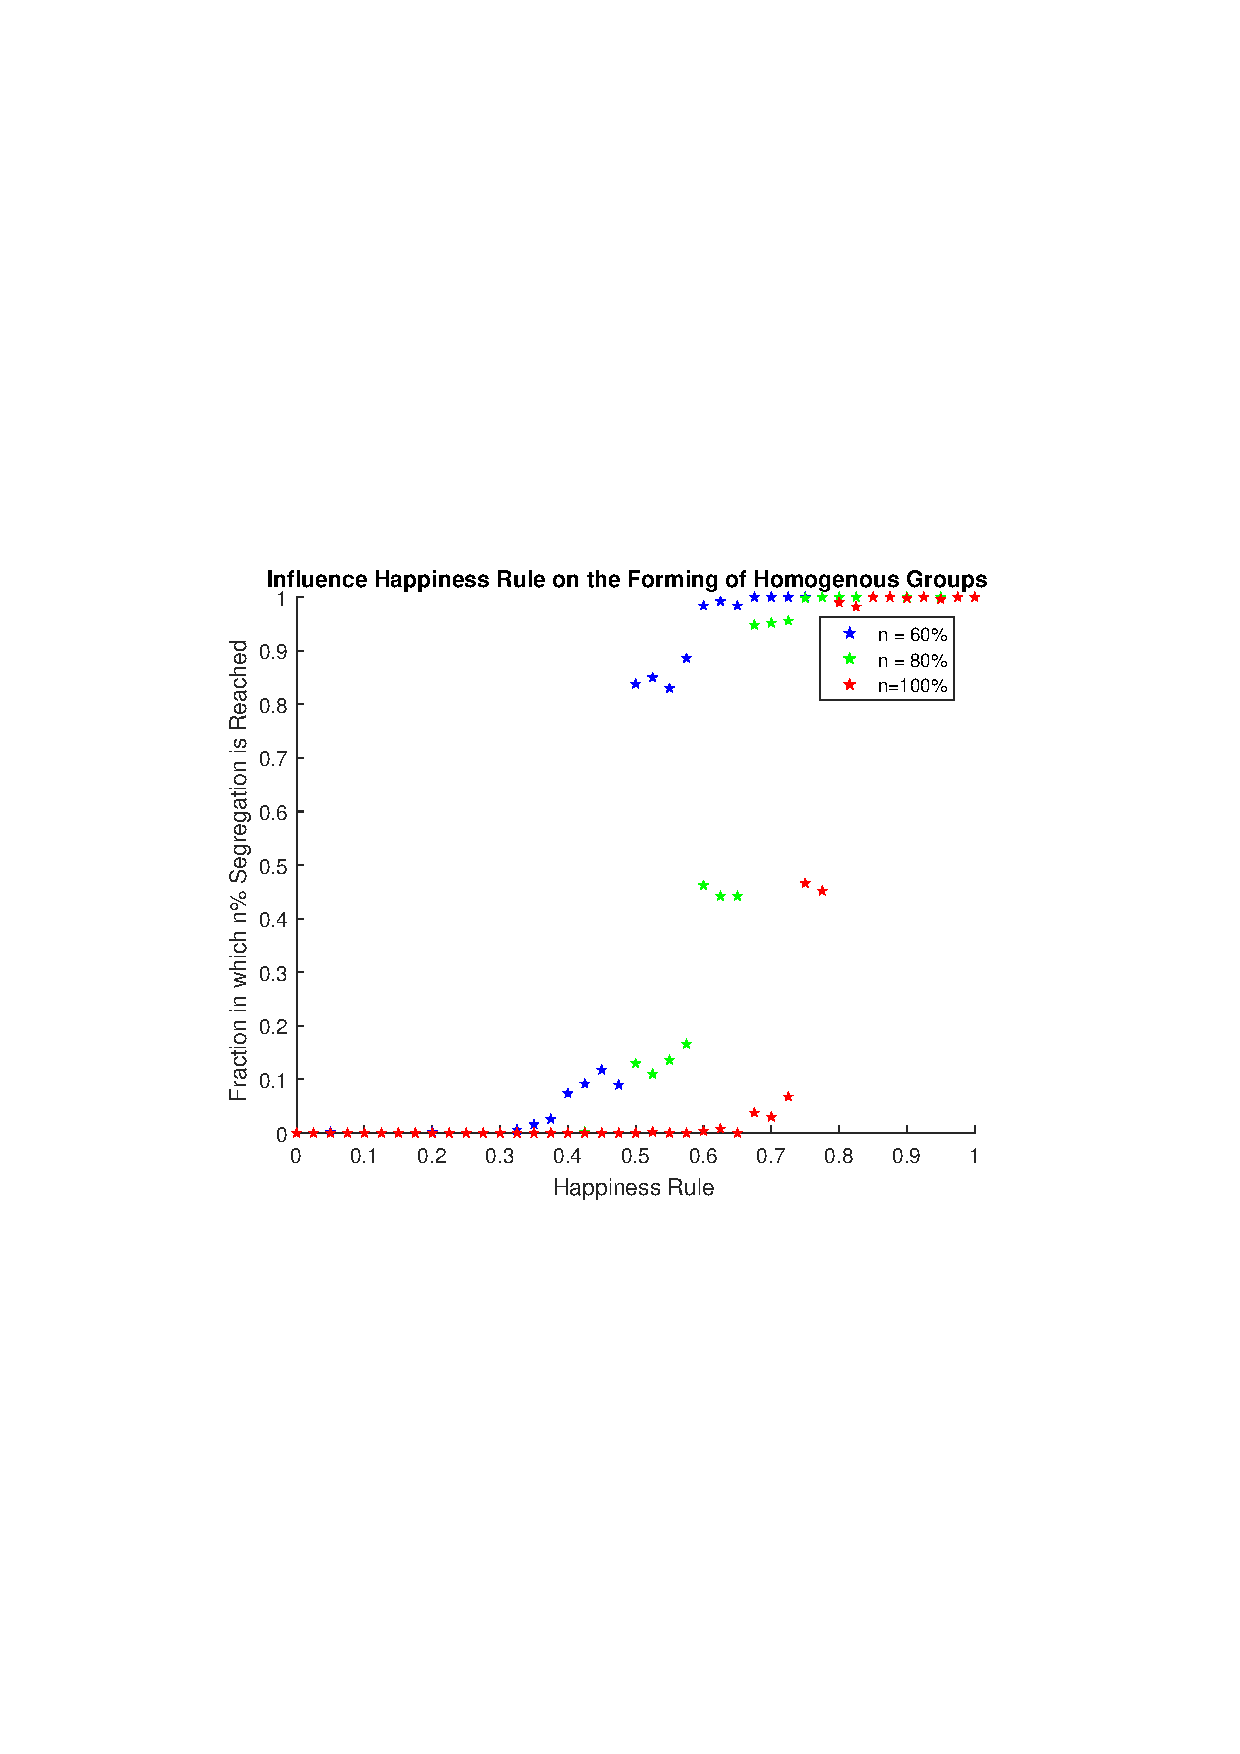
\includegraphics{happy_segr_60_80_100.pdf}
>>>>>>> 0cb6cf99d2ea0e6d2392a800ee71f7cf80f50400
    \caption{a nice plot}
    \label{fig:mesh1}
\end{figure}
\end{document}